% shavar — comparative notes on seven implementations of SHA-256.
%
% Build:  latexmk -pdf shavar.tex     (biber is used for the bibliography)
% Tested: doc/test_doc.sh checks that this builds and that no reference
%         resolves to ??.
\documentclass[11pt,a4paper]{article}

\usepackage[T1]{fontenc}
\usepackage[utf8]{inputenc}
\usepackage{lmodern}
\usepackage[margin=2.4cm]{geometry}
\usepackage{microtype}
\usepackage{booktabs}
\usepackage{array}
\usepackage{longtable}
\usepackage{amsmath,amssymb}
\usepackage{tikz}
\usepackage{xcolor}
\usepackage{listings}
\usepackage{enumitem}
\usepackage{url}
\usetikzlibrary{arrows.meta,positioning,fit,backgrounds,calc,decorations.pathreplacing}

\usepackage[backend=biber,style=numeric,backref=true,sorting=nyt]{biblatex}
\addbibresource{refs.bib}

\usepackage[colorlinks=true,linkcolor=linknavy,citecolor=citegreen,
            urlcolor=linknavy,breaklinks=true]{hyperref}

% ---- palette -------------------------------------------------------------
% One meaning per colour, used consistently in prose, tables and diagrams.
\definecolor{linknavy}{HTML}{1F4E79}
\definecolor{citegreen}{HTML}{2E6B4F}
\definecolor{trackA}{HTML}{1F6FB2}    % the A track, everywhere
\definecolor{trackE}{HTML}{B23A1F}    % the E track, everywhere
\definecolor{crossAE}{HTML}{6A1FB2}   % the single A->E edge, everywhere
\definecolor{softgrey}{HTML}{6B6B6B}
\definecolor{panelbg}{HTML}{F4F6F8}

\lstdefinestyle{sv}{
  basicstyle=\ttfamily\footnotesize,
  keywordstyle=\color{linknavy}\bfseries,
  commentstyle=\color{softgrey}\itshape,
  breaklines=true, frame=single, rulecolor=\color{softgrey!40},
  backgroundcolor=\color{panelbg}, showstringspaces=false,
  xleftmargin=0.5em, framexleftmargin=0.5em,
}
\lstset{style=sv}

\newcommand{\lang}[1]{\textsf{#1}}
\newcommand{\code}[1]{\texttt{#1}}

\title{\textbf{shavar}\\[0.3em]
  \large Seven implementations of SHA-256, written as a two-dimensional
  recurrence\\[0.4em]
  \normalsize What each language makes natural, and what it makes hard}
\author{}
\date{9 August 2026}

\begin{document}
\maketitle

\begin{abstract}
\noindent
SHA-256 is normally presented as eight working registers that shuffle on every
round. Six of those eight assignments are pure copies. Removing them leaves two
coupled recurrences with a lookback of four, which is both smaller to write and
closer to the object that cryptanalysis actually reasons about. This note
reports on implementing that formulation seven times --- in C99, Lean~4,
Python, Perl, Scheme, JavaScript and shell --- under a rule of \emph{core
language only, no libraries}, and on what the exercise revealed about the
languages rather than about the algorithm. All seven agree byte-for-byte on
every intermediate value, which is the evidence that the comparison is between
seven correct programs rather than seven different bugs.
\end{abstract}

\tableofcontents
\bigskip

% =========================================================================
\section{The reformulation}
\label{sec:reform}

FIPS 180-4~\cite{fips180-4} defines the compression function over eight
variables $a \ldots h$, updated each round as
%
\begin{align*}
T_1 &= h \boxplus \Sigma_1(e) \boxplus \mathrm{Ch}(e,f,g) \boxplus K_t \boxplus W_t, &
T_2 &= \Sigma_0(a) \boxplus \mathrm{Maj}(a,b,c),\\
h &\leftarrow g,\quad g \leftarrow f,\quad f \leftarrow e,\quad e \leftarrow d \boxplus T_1, &
d &\leftarrow c,\quad c \leftarrow b,\quad b \leftarrow a,\quad a \leftarrow T_1 \boxplus T_2,
\end{align*}
%
where $\boxplus$ is addition modulo $2^{32}$. Six of those eight assignments
move a value without changing it. They are not computation; they are a shift
register written out longhand.

Name the two computed sequences and index them by round. With
$A_{-1}\!=\!H_0, A_{-2}\!=\!H_1, A_{-3}\!=\!H_2, A_{-4}\!=\!H_3$ and
$E_{-1}\!=\!H_4, \ldots, E_{-4}\!=\!H_7$, the whole compression is
%
\begin{equation}\label{eq:2d}
\fbox{$\displaystyle
\begin{aligned}
T_1[t] &= E_{t-4} \boxplus \Sigma_1(E_{t-1}) \boxplus \mathrm{Ch}(E_{t-1},E_{t-2},E_{t-3}) \boxplus K_t \boxplus W_t \\
T_2[t] &= \Sigma_0(A_{t-1}) \boxplus \mathrm{Maj}(A_{t-1},A_{t-2},A_{t-3}) \\
E_t    &= A_{t-4} \boxplus T_1[t] \\
A_t    &= T_1[t] \boxplus T_2[t]
\end{aligned}$}
\end{equation}
%
The correspondence with the standard form is exactly
$a = A_{t-1}$, $b = A_{t-2}$, $c = A_{t-3}$, $d = A_{t-4}$ and
$e = E_{t-1}, \ldots, h = E_{t-4}$: the eight registers are two sliding
windows of width four. Figure~\ref{fig:tracks} draws one round.

This is not a new observation --- it is how the function is handled in the
cryptanalytic literature --- but it is rarely how it is \emph{implemented}, and
implementing it this way turns out to change the character of the code in every
language. Section~\ref{sec:perlang} is mostly about that.

\subsection*{Two properties worth having in view}

\begin{description}[leftmargin=1.4em,style=nextline]
\item[The state \emph{is} the history.] Keeping all of $A_{-4..63}$ and
  $E_{-4..63}$ costs 136 words per block. Every intermediate value is then
  addressable after the fact at no extra cost, which is what makes the code
  usable as an instrument rather than only as a hash.
\item[The tracks are not symmetric.] $A_t$ reads the $E$ history at three
  points (through $\mathrm{Ch}$) plus $E_{t-4}$; but $E_t$ reads the $A$
  history at exactly one point, $A_{t-4}$. That single edge is the only path
  by which the $A$ track influences the $E$ track at all. It is drawn thick and
  violet in Figure~\ref{fig:tracks} because it is easy to miss in the algebra
  and hard to miss in a picture.
\end{description}

% ---- Figure 1: one round of the recurrence -------------------------------
\begin{figure}[t]
\centering
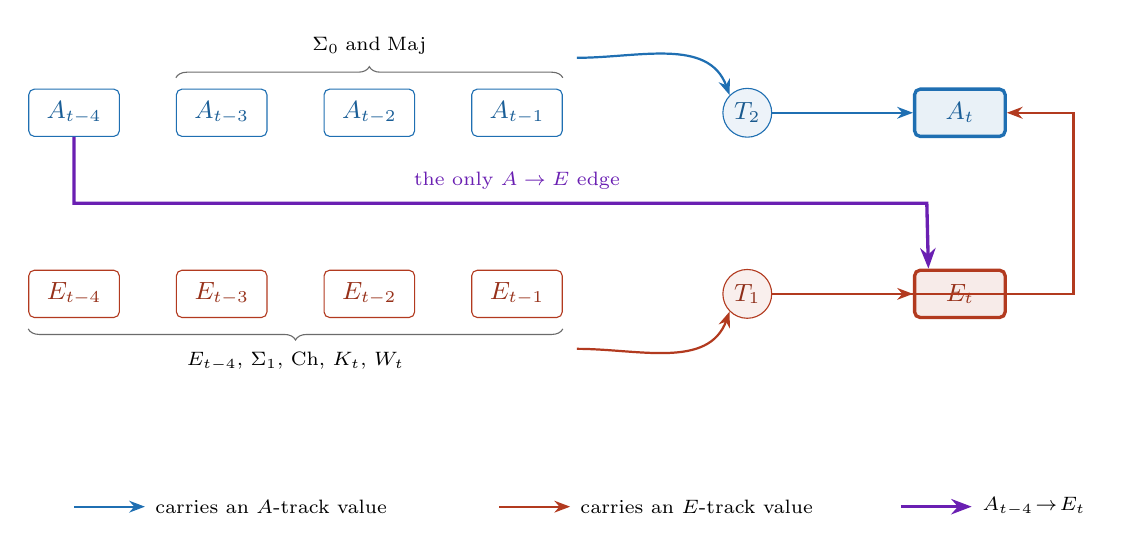
\begin{tikzpicture}[
  x=1.5cm, y=1.15cm,
  cell/.style={draw, rounded corners=2pt, minimum width=1.15cm,
               minimum height=0.6cm, font=\ttfamily\small, fill=white,
               inner sep=1pt},
  acell/.style={cell, draw=trackA, text=trackA!85!black},
  ecell/.style={cell, draw=trackE, text=trackE!85!black},
  op/.style={draw, circle, minimum size=0.62cm, inner sep=0pt, font=\small},
  aflow/.style={-{Stealth[length=2mm]}, trackA, thick},
  eflow/.style={-{Stealth[length=2mm]}, trackE, thick},
  cross/.style={-{Stealth[length=2.6mm]}, crossAE, line width=1.2pt},
  brc/.style={decorate, decoration={brace, amplitude=4pt}, softgrey},
]

% --- the A row (top) and E row (bottom). The horizontal corridor at y=1
% --- between them is kept completely clear so the one A->E edge can run
% --- through it without crossing anything else.
\node[acell] (a4) at (0,2)    {$A_{t-4}$};
\node[acell] (a3) at (1.25,2) {$A_{t-3}$};
\node[acell] (a2) at (2.5,2)  {$A_{t-2}$};
\node[acell] (a1) at (3.75,2) {$A_{t-1}$};
\node[acell, fill=trackA!10, very thick] (a0) at (7.5,2) {$A_{t}$};

\node[ecell] (e4) at (0,0)    {$E_{t-4}$};
\node[ecell] (e3) at (1.25,0) {$E_{t-3}$};
\node[ecell] (e2) at (2.5,0)  {$E_{t-2}$};
\node[ecell] (e1) at (3.75,0) {$E_{t-1}$};
\node[ecell, fill=trackE!10, very thick] (e0) at (7.5,0) {$E_{t}$};

\node[op, draw=trackA, fill=trackA!8, text=trackA!80!black] (T2) at (5.7,2) {$T_2$};
\node[op, draw=trackE, fill=trackE!8, text=trackE!80!black] (T1) at (5.7,0) {$T_1$};

% --- which cells feed which accumulator, shown as a span rather than as
% --- one arrow per cell: seven converging arrows cannot be drawn without
% --- crossing the boxes they start from.
\draw[brc] ($(a3.north west)+(0,0.12)$) -- ($(a1.north east)+(0,0.12)$)
  node[midway, above=5pt, font=\scriptsize, black]
  {$\Sigma_0 \;\text{and}\; \mathrm{Maj}$};
\draw[aflow] ($(a1.north east)+(0.12,0.34)$) to[out=0,in=110] (T2.north west);

\draw[brc] ($(e1.south east)+(0,-0.12)$) -- ($(e4.south west)+(0,-0.12)$)
  node[midway, below=5pt, font=\scriptsize, black]
  {$E_{t-4}$, $\Sigma_1$, $\mathrm{Ch}$, $K_t$, $W_t$};
\draw[eflow] ($(e1.south east)+(0.12,-0.34)$) to[out=0,in=-110] (T1.south west);

% --- outputs. A_t = T1 + T2, so T1 reaches A_t as well; it is routed round
% --- the right-hand side so that it never enters the corridor.
\draw[aflow] (T2) -- (a0);
\draw[eflow] (T1) -- (e0);
\draw[eflow] (T1.east) -- ++(2.55,0) |- (a0.east);

% --- THE single A -> E edge, straight down the clear corridor.
% Down out of A_{t-4}, along the empty corridor, and into the TOP of E_t.
% Nothing else may be drawn between y=1 and the A row at x=7.5, or the edge
% would read as A_t -> E_t, which is not what it is.
% The drop is offset left of centre so that it cannot be misread as
% descending from A_t, which sits directly above E_t.
\draw[cross] (a4.south) -- (0,1) -- (7.22,1) -- ([xshift=-4mm]e0.north);

\node[font=\scriptsize, crossAE] at (3.75,1.25) {the only $A\rightarrow E$ edge};

% --- legend --------------------------------------------------------------
\begin{scope}[shift={(0,-2.35)}]
  \draw[aflow] (0,0) -- ++(0.6,0)
    node[right, font=\scriptsize, black] {carries an $A$-track value};
  \draw[eflow] (3.6,0) -- ++(0.6,0)
    node[right, font=\scriptsize, black] {carries an $E$-track value};
  \draw[cross] (7.0,0) -- ++(0.6,0)
    node[right, font=\scriptsize, black] {$A_{t-4}\!\rightarrow\!E_t$};
\end{scope}
\end{tikzpicture}
\caption{One round of the recurrence of Equation~\eqref{eq:2d}. A box is a
32-bit word; a circle is an accumulator; an arrow is a word flowing into an
arithmetic step. Blue arrows read the $A$ track, red arrows read the $E$
track, and the single violet edge $A_{t-4} \rightarrow E_t$ is the one place
where the $A$ track feeds the $E$ track. Advancing a round shifts both rows
one cell to the left; nothing is copied.}
\label{fig:tracks}
\end{figure}

% =========================================================================
\section{The seven implementations at a glance}
\label{sec:glance}

Every implementation obeys the same command-line contract, so any one can be
diffed against any other not merely on the final digest but on the full
per-round interior: $W$, $A$, $E$, $T_1$, $T_2$ for all 64 rounds. That is
what \emph{agree} means in Table~\ref{tab:glance} --- 344 identical lines of
trace, not 64 identical hex characters.

\begin{table}[h]
\centering
\small
\begin{tabular}{@{}llrrl@{}}
\toprule
\textbf{Language} & \textbf{Runtime} & \textbf{Lines} & \textbf{ms/block} & \textbf{Character of the port} \\
\midrule
C99        & clang 17           &  315 & 0.0005 & the reference; zero allocations \\
Lean 4     & 4.32.2             & 1851 & ---    & implementation \emph{and} proofs \\
Python     & 3.9.6              &  776 & 0.63   & operator overloading, generators \\
Perl       & 5.34.1             &  539 & 0.16   & \code{vec()}, \code{pack}, negative indices \\
Scheme     & chibi 0.12 (R7RS)  & 1106 & 6.6    & \code{syntax-rules}; no bitwise ops exist \\
JavaScript & JavaScriptCore     &  787 & 0.017  & \code{Uint32Array}; no integer type \\
shell      & bash 3.2 / zsh 5.9 &  811 & 14.9 / 2.4 & builtins only; no subshells \\
\bottomrule
\end{tabular}
\caption{Line counts are the implementation file only, excluding tests and
excluding the Lean proofs' share. Timings are per 512-bit block on an
M-series Mac with other work running concurrently; they are honest to about a
factor of two and are included for their \emph{ratios}, not their absolute
values. C is roughly \(3\times10^{4}\) times faster than bash.}
\label{tab:glance}
\end{table}

The line counts deserve a caveat before anyone reads them as a brevity
ranking. Every file here is heavily commented for a reader who does not know
the language, which was a project requirement; comment density varies more
than code density does. C is the shortest partly because it is expressive for
this task and partly because \code{uint32\_t} does for free what four other
languages spend thirty lines simulating.

% =========================================================================
\section{Where the language helps, and where it fights}
\label{sec:perlang}

\subsection{The one problem every language except two has}

SHA-256 is defined on 32-bit words with wraparound. Exactly two of the seven
languages have that type natively: C (\code{uint32\_t}) and Lean
(\code{BitVec 32}). The other five must simulate it, and \emph{how} they
simulate it is the single largest stylistic difference between the ports.

\begin{itemize}[leftmargin=1.3em]
\item \textbf{Python} confines the mask to one place by giving a
  \code{Word32} class overloaded arithmetic. The round body then reads like
  Equation~\eqref{eq:2d} instead of like the equation plus fourteen
  \code{\& 0xFFFFFFFF}. A genuine payoff: \code{\textasciitilde x} on a Python
  integer is negative, and masking inside the constructor turns it into the
  correct 32-bit complement for free.
\item \textbf{JavaScript} has no integer type at all. Bitwise operators
  coerce to \emph{signed} \code{int32}, so \code{0xFFFFFFFF | 0} is $-1$ and
  the natural big-endian assembly goes negative on any high byte.
  \code{>>>\,0} is the only unsigned-producing operator. The clean fix is
  \code{Uint32Array}, which is core language, not a library: every store
  passes through \code{ToUint32}, giving real machine-word wraparound.
\item \textbf{Perl} and \textbf{shell} mask by hand at every site. Both are
  64-bit signed underneath, so a missed mask is a silently wrong digest far
  downstream with no type to catch it.
\item \textbf{Scheme} has the same problem plus a larger one, below.
\end{itemize}

\subsection{R7RS-small has no bitwise operations}

Not ``no rotate'' --- no \code{and}, \code{or}, \code{xor}, or shift, at all.
The base library of R7RS~\cite{r7rs} simply does not include them. A portable
Scheme implementation of a function \emph{defined} in terms of those
operations must therefore rebuild the entire layer from \code{quotient} and
\code{remainder}. This is the single largest structural cost imposed by any
language in the set: roughly forty lines and an eightfold slowdown before the
algorithm proper begins. The port handles it with \code{cond-expand} to pick
up host primitives where they exist, and \emph{tests both paths}, since a
fallback that is never executed is a fallback that does not work.

\subsection{The lookback window: four ways to say $A_{t-4}$}

Equation~\eqref{eq:2d} indexes backwards from the current round. Each language
expresses that differently, and the differences are instructive:

\begin{longtable}{@{}p{2.3cm}p{12.3cm}@{}}
\toprule
\textbf{Language} & \textbf{How $A_{t-4}$ is written} \\
\midrule
\endhead
Python, Perl &
  \code{A[-4]}, literally. If the list holds exactly the history so far, the
  language's own negative indexing \emph{is} the lookback window and no index
  arithmetic appears anywhere. This is the closest any port gets to the
  equation. It carries a trap: the append order matters
  (\code{E.append} must precede \code{A.append}), and once the list stops
  growing, \code{A[-4]} silently means $A_{60}$ instead. Python's port needs a
  separate accessor class for the finished trace for exactly this reason ---
  the best feature in the file is also the most dangerous. \\
\addlinespace
C, JavaScript &
  \code{A[4 + t]}, with the array offset by four so that $t$ may be negative.
  Explicit, checkable, and needs a comment warning about the off-by-one. \\
\addlinespace
Scheme &
  A \code{syntax-rules} macro, so the four lines of Equation~\eqref{eq:2d} are
  the literal source text with the indexing pushed into the macro. This is the
  only port where the spec and the code are the same characters. Macro hygiene
  makes it safe in a way a C preprocessor macro would not be. \\
\addlinespace
Lean &
  A \code{Vector} whose length is part of its type, so an out-of-range index
  is not a runtime error but a program that does not compile. \\
\addlinespace
shell &
  Indexed arrays and a global out-parameter, because shell functions return
  only an exit status. There is no abstraction available to hide it behind. \\
\bottomrule
\end{longtable}

\subsection{Three findings that surprised us}

\paragraph{JavaScript cannot return an exit code.}
The language has no notion of a process. Under \code{jsc}, Safari's engine,
\code{quit()} \emph{ignores its argument and always exits 0}; the only nonzero
status it ever produces is 3, for an uncaught exception. A three-valued exit
contract that every other language gets for free therefore required making the
CLI a shell/JavaScript polyglot whose first two lines re-invoke the engine and
translate a sentinel. This is a property of the host, not of the language, but
it is exactly the kind of thing a portability comparison exists to surface.

\paragraph{Shell is not one data point.}
The same source runs about \emph{four to six times faster under zsh 5.9 than
under bash 3.2.57}. Meanwhile the micro-optimisation one would expect to
matter --- collapsing each round into a single comma expression rather than a
dozen \code{(( ))} statements --- is worth nothing measurable in either shell.
Shell arithmetic cost lives in operators and variable lookups, not statement
dispatch. Both facts were measured after being predicted wrongly.

\paragraph{An alias broke a proof tactic, silently.}
In Lean, \code{abbrev Word := BitVec 32} --- fully reducible and apparently
harmless --- makes \code{bv\_decide} fail. The alias survives inside instance
arguments of the elaborated term, the bit-blaster matches those syntactically,
and the tactic then reports a \emph{spurious counterexample} rather than an
error. Failing ``successfully'' is the worst possible failure mode for a
verification tool, and the fix was to delete the alias and write
\code{BitVec 32} everywhere.

% =========================================================================
\section{What is proved, and what is merely tested}
\label{sec:verification}

These are different kinds of evidence and the distinction is worth keeping
sharp. Table~\ref{tab:verif} states which is which.

\begin{table}[h]
\centering
\small
\begin{tabular}{@{}clp{7.3cm}l@{}}
\toprule
& \textbf{Claim} & \textbf{Evidence} & \textbf{Status} \\
\midrule
V1 & 2D form $\equiv$ 8-register form & Lean, by induction over rounds; lifted to block and whole-hash level & proved, kernel-only \\
V2 & Bitwise identities (Ch, Maj, $\Sigma$, $\sigma$) & 31 theorems; 11 kernel-only, 20 via \code{bv\_decide} & proved \\
V3 & Padding lands on a 512-bit multiple & Lean, arithmetic on $L \bmod 512$ & proved, kernel-only \\
V4 & Padding is injective & Lean, given well-formedness & proved, kernel-only \\
V5 & Agreement with FIPS 180-4 & Known-answer vectors & tested \\
V6 & The seven agree with each other & Full per-round traces, swept bit lengths & tested \\
\bottomrule
\end{tabular}
\caption{There is no \code{sorry} anywhere in \texttt{lean/}. V1's proof is
\emph{kernel-only}: \code{\#print axioms} reports \code{[propext, Quot.sound]}
and nothing else.}
\label{tab:verif}
\end{table}

\paragraph{On trusting \code{bv\_decide}.}
The tactic bit-blasts a goal to CNF, calls a bundled CaDiCaL, and checks the
returned LRAT certificate inside Lean~\cite{boving2025bvdecide}. The SAT
solver is \emph{not} trusted. The certificate check runs as compiled native
code, so the Lean compiler is. On this toolchain that shows up as a
per-theorem axiom \code{<name>.\_native.bv\_decide.ax\_N}, which
\code{\#print axioms} makes visible --- and which the build prints on every
run rather than asserting cleanliness in prose. Notably, the two identities
that matter most are proved \emph{twice}, once by \code{bv\_decide} and once
by case analysis on bit positions, and the second route needs no compiler
trust at all.

\paragraph{An honest gap.} V3 and V4 are proved about an abstract bit-level
padding function, and a separate lemma links the concrete byte-level padder's
\emph{length} to it. What is \emph{not} proved is that the byte padder emits
the same bit string as the abstract one, only that it emits one of the right
length. That gap is real and is marked as such in the source.

\paragraph{Why V5 and V6 do not subsume one another.}
V5 catches a shared misreading of the standard; V6 catches a transcription
slip in one language --- and because it compares traces, it names the round
where the slip happened. Seven implementations could agree with each other and
all be wrong, or all match NIST on byte-aligned input and diverge at $L = 5$.

\paragraph{The limit of external validation.}
OpenSSL, LibreSSL, \code{shasum} and \code{sha256sum} all hash whole bytes
only. \emph{No external oracle on a normal machine can validate a message
whose length is not a multiple of eight.} For those cases the evidence is
cross-implementation agreement plus NIST's bit-oriented CAVP
vectors~\cite{nistcavp}, and the repository says so rather than letting
seven-way agreement stand in for external validation.

Prior work is worth naming here for scale: Appel's machine-checked proof of
the OpenSSL C implementation of SHA-256~\cite{appel2015sha} verifies a real
optimised C program against a functional specification in Coq, which is a
substantially harder undertaking than anything in this repository. What
\path{lean/} proves is the correctness of a \emph{reformulation}, not of an
optimised implementation.

% =========================================================================
\section{Using it as an instrument}

The reason for keeping the whole trajectory (\S\ref{sec:reform}) is that the
intended reader is studying the function, not hashing a file. Every
implementation therefore also offers the compression function on a
caller-supplied chaining value and for a reduced number of rounds --- neither
reachable through a normal hashing API, and both prerequisites for free-start
and reduced-round analysis.

Two structural facts the formulation makes visible, and which the code keeps
separately addressable rather than fusing into one expression:

\begin{description}[leftmargin=1.4em,style=nextline]
\item[The linear/nonlinear split.] $\oplus$, rotation and shift are
  $\mathrm{GF}(2)$-linear, hence so are $\Sigma_0,\Sigma_1,\sigma_0,\sigma_1$.
  The nonlinearity lives entirely in $\mathrm{Ch}$, $\mathrm{Maj}$, and the
  carries of $\boxplus$. Replace those and the function collapses to an affine
  map over $\mathrm{GF}(2)^{256}$.
\item[Bit-slices are coupled only by carries.] $\mathrm{Ch}$, $\mathrm{Maj}$
  and $\oplus$ act bit-position-wise; rotations permute positions without
  mixing them. The \emph{only} operation moving information from bit $i$ to
  bit $j > i$ is the carry in $\boxplus$ --- and it moves one way, towards the
  most significant bit. Replace every $\boxplus$ with $\oplus$ and SHA-256
  decomposes into 32 independent one-bit ciphers. This asymmetry is why
  low-order differences are cheap to control and high-order ones are not.
\end{description}

The browser page in \path{js/index.html} exists to make this visible rather
than merely stated: it steps through rounds forwards and backwards, draws the
order-4 window and the single $A\!\rightarrow\!E$ edge of
Figure~\ref{fig:tracks} on live data, renders words as individual bits, and in
diff mode shows a one-bit input difference avalanching across 64 rounds as a
Hamming-weight curve.

% =========================================================================
\section{Conclusions}

\begin{enumerate}[leftmargin=1.5em]
\item \textbf{The reformulation is worth it.} In every language the round body
  became four lines with no permutation to get wrong, and the six copy
  assignments of the standard form vanished entirely. In Lean the equivalence
  to the standard form is \emph{definitional} for a single round --- which is
  the formal statement of ``the register shuffle was never computation''.
\item \textbf{The decisive language feature was not what we expected.} It was
  not macros, or pattern matching, or types. It was whether the language has a
  32-bit unsigned integer. Two do; the other five spend their idiom budget
  simulating one, and that choice --- wrapper class, typed array, or manual
  masking --- shapes the rest of the file more than anything else.
\item \textbf{Negative indexing is the sleeper feature.} Python and Perl
  transcribe the recurrence with no index arithmetic at all, because a list's
  negative indices already \emph{are} a lookback window. It is also the most
  dangerous feature in both files.
\item \textbf{Seven-way trace agreement is a strong instrument and a weak
  oracle.} It localises a disagreement to a round and a register, which no
  digest comparison can do. It cannot tell you all seven are not wrong
  together, which is what the NIST vectors are for.
\end{enumerate}

\printbibliography[heading=bibintoc]

\end{document}
